%!Tex Program = xelatex
%\documentclass[a4paper]{article}
\documentclass[a4paper]{ctexart}
\usepackage{xltxtra}
%\setCJKmainfont{Noto Serif CJK SC}
%\setCJKmainfont{AR PL UMing CN:style=Light}
%\setmainfont[Mapping=tex-text]{AR PL UMing CN:style=Light}
%\setmainfont[Mapping=tex-text]{AR PL UKai CN:style=Book}
%\setmainfont[Mapping=tex-text]{WenQuanYi Zen Hei:style=Regular}
%\setmainfont[Mapping=tex-text]{WenQuanYi Zen Hei Sharp:style=Regular}
%\setmainfont[Mapping=tex-text]{AR PL KaitiM GB:style=Regular} 
%\setmainfont[Mapping=tex-text]{AR PL SungtiL GB:style=Regular} 
%\setmainfont[Mapping=tex-text]{WenQuanYi Zen Hei Mono:style=Regular} 

\usepackage{listings}
\usepackage{xcolor}
\usepackage{graphicx}
\usepackage{amsmath}
\usepackage{amsthm}
\usepackage{amssymb}
\usepackage{mathrsfs}
\definecolor{codegreen}{rgb}{0,0.6,0}
\definecolor{codegray}{rgb}{0.5,0.5,0.5}
\definecolor{codepurple}{rgb}{0.58,0,0.82}
\definecolor{backcolour}{rgb}{0.95,0.95,0.92}

\renewcommand{\thefigure}{\arabic{section}.\arabic{figure}}

\lstdefinestyle{mystyle}{
    backgroundcolor=\color{backcolour},   
    commentstyle=\color{codegreen},
    keywordstyle=\color{magenta},
    numberstyle=\tiny\color{codegray},
    stringstyle=\color{codepurple},
    basicstyle=\ttfamily\footnotesize,
    breakatwhitespace=false,         
    breaklines=true,                 
    captionpos=b,                    
    keepspaces=true,                 
    numbers=left,                    
    numbersep=5pt,                  
    showspaces=false,                
    showstringspaces=false,
    showtabs=false,                  
    tabsize=2
}

\lstset{style=mystyle}

\newcommand{\hl}[1]
{\noindent {\bf {#1}}}

% 创建定理环境  
\newtheorem{theorem}{定理}  

\theoremstyle{definition}  
\newtheorem{definition}{定义}[section]

\theoremstyle{definition}  
\newtheorem{example}{例}[section]  


\title{数据结构和算法}
\author{王何宇}
\date{}
\begin{document}
\maketitle
\pagestyle{empty}


\setcounter{section}{5}
\section{优先队列, 堆 (Priority Queues, Heap)}
排队的一个基本原则是, 不能插队. 但是在讨论算法时, 这并不是不可突破的.
想象一下一个大家都碰到过的场景, 你去银行取 200 块钱, 然后你身后大概 20
个人有着类似的需求, 但你前面一个贱人, 要把 200 块钱转给 200 个帐号
... 因此如果一个队列中积累了较多的工作, 显然优先执行工作量较小的请求是
一个高效率系统的刚性需求.

\subsection{基本模型}

针对这种需求, 人们提出了优先队列(priority queue)这种 ADT 概念. 并要求
至少提供两个基本操作:

\begin{itemize}
\item {\bf insert}: 入队, 正经操作, 没啥好说的;
\item {\bf deleteMin}: 出队, 但每次出队的总是队列中最小的元素; 
\end{itemize}

\subsection{简单实现}

显然, 这个结构同样要求队列中的元素有一定的序关系. 尽管可以考虑的实现方
式有很多, 比如链表(List), 或者平衡树. 但是前者效率较低, 后者则过于复杂.
以至于优先队列这个名字, 很多时候默认就指向一种具体的数据结构: 这一讲我
们介绍一种实现非常简单的结构: {\bf 二叉堆(Binary Heap)}.  它不但支持上
面两种基本操作, 而且最坏可能性下, 复杂度也是 $\Theta(\log n)$. 甚至对
于连续的 \verb|insert| 操作, 其平均效率是 $\Theta(1)$.

\subsection{二叉堆 (Binary Heap)}

\noindent{\bf 二叉堆(binary heap)} 一个二叉堆是一个完全二叉树
(complete binary tree), 且其最后一层叶子的缺少, 只能在右边. 此外, 堆中
任何一个除根节点以外的节点的值, 必须小于其左右孩子节点的值.

容易看出, 一个堆的节点总数 $n$ 必然有
$$
2^h \leq n \leq 2^{h + 1} - 1,
$$
因此其高度 $h = \lfloor \log n \rfloor$.

\subsubsection{结构性质}

堆的另一个重要性质是, 这种结构极其有规律, 因此我们不需要真的构建二叉树,一
般用数组就可以快速实现. 比如书上建议, 第 $k$ 层的全部节点, 依次存放在
数组的第 $2^{k-1} \sim 2^{k} - 1$ 位置. $k$ 从 $1$ 开始计算. 这样堆中
从左到右, 至上而下的第 $i$ 个节点, 它存放在数组中的下标是 $i$, 而它的
左孩子必然是数组下标 $2i$ 的元素, 右孩子则是 $2i + 1$, 父节点是
$\lfloor i / 2\rfloor$. 数组中的 $0$ 下标元素暂时空在那里. 因此, 尽管
堆在逻辑上是一棵满二叉树, 但实际上, 它的一切基本操作, 都只涉及数组.

\subsubsection{堆的有序性}

现在我们再考虑到堆的有序性, 也就是除根节点以外, 任何节点的父节点的
\verb|key|, 都必然小于等于自己的 \verb|key|. 显然, 如果能正确维持堆的
性质, 那么整个堆中的最小元素, 必然是它的根节点. 现在我们来考虑如何在两
个基本操作下, 始终保持这些基本性质. Fig 6.5 的右图是一个(看上去很像但)
不是 heap 的例子, 虚线标出了对序关系的违背.


\subsubsection{基本操作}
\noindent{\bf \verb|insert|}
首先我们将新元素插入到数组的下一个空余位置(假设数组足够长). 这样既可以
保持堆是满二叉树, 最后一层叶子从左到右紧密排列, 同时也考虑到这样的插入
对数组是 $\Theta(1)$ 的(记录了尾部的下标). 但是插入之后, 我们可能破坏
了堆的有序性, 这个新插入的元素值, 可能小于它的父节点. 因此我们要做判断,
如果它当前所在节点的父节点的值比它大, 我们需要交换二者的值.  这个动作
称为升堆(percolate up). 我们每插入一个新元素在堆的末尾, 都需要不断地升
堆, 直至达到正确的位置, 或者直到升到根(此时它是新的最小元素).  显然,
在一次独立的插入中, 升堆的最大执行次数是 $h = \Theta(\log n)$.

按照这种思路, 我们有可能要做 $h$ 次交换, 而 $1$ 次交换本身是需要 $3$次
赋值操作的, 因此最坏可能下, 要 $3h$ 次赋值操作. 而书上建议可以利用数组
的 $0$ 位置做缓存(其实就是只要一个缓存, 既然它空着). 在需要交换的时候,
我们每次都只把父节点往下移动一层(每次移动 $1$ 次赋值操作). 这样当我们
完成移动之后, 最坏可能下, 也只需要 $h + 1$ 次赋值操作. 对于堆这样的基
础核心算法和结构, 有必要精打细算. 具体的算法细节可参见书上的代码 Fig
6.8. 这里注意一个细节, 当数组空间用完时, 我们会加倍数组长度. 这一般为
导致全部数据的复制, 是一个$\Theta(n)$ 的代价. 这里课本上基础存储结构是
\verb|std::vector|. 参见 Fig 6.4.

\noindent{\bf \verb|deleteMin|}

根就是最小元素, 问题是当删除根以后, 如何填充其空位, 并保持堆性质. 一个
偷懒的思路是, 把堆(数组)的最后一个元素塞到这个位置, 然后把它降堆
(precolate down)到合适的位置. 这里对一个节点的降堆, 就是比较它和它的两
个孩子, 如果它比小的孩子大, 就把它和小的孩子交换. 同样地, 我们仍然想尽
量减少赋值运算, 和升堆一样, 我们先把可能的位置空出来, 然后不断地把这个
空位下移, 直到找到正确的空位, 然后把最后一个元素填进去就行了. 这里我们
连缓存都不需要, 因为本来就是一个元素减少的过程.

因此我们看到堆的实现非常简单, 但仍然有一些细节需要注意. 比如最后一个叶
子的父亲是可能只有一个左孩子的 (Fig, 6.11), 因此不能总是假设所有非叶子
节点都有两个孩子. 这一点在实施的时候要小心. 要每个节点都做额外的判定
(课本上 Fig 6.12中的第 40 行). 

\subsubsection{其他堆操作}

注意堆只有很基础的序信息. 因此一般是无法准确定位一个具体元素的位置的.
比如我们可以以 $\Theta(1)$ 时间找到最小元素, 但是寻找最大元素确是一个
$\Theta(n)$ 的操作. 因为它可能在任何一个叶子出现, 最坏可能性下, 叶子总
数是 $n / 2$. 所以除非有另外的快速索引, 比如另建了一个哈希表用于定位.
否则下面的额外操作, 是无法以 $\Theta(\log n)$ 效率实现的.

\begin{itemize}
\item \verb|decreaseKey(p, D)|: 将位置 \verb|p| 处的 \verb|key|, 减少
  \verb|D|. 因为可能破坏了序关系, 需要做升堆处理. (赤裸裸的插队! 氪金玩家, VIP, ...)

\item \verb|increaseKey(p, D)|: 将位置 \verb|p| 处的 \verb|key|, 增加
  \verb|D|. 可能需要做降堆. (这又是得罪了谁?)

\item \verb|remove(p)|: 删除一个指定位置 \verb|p| 的节点.
\end{itemize}
以上操作可能有助于管理员管理它的队列.

\noindent{\bf \verb|buildHeap|}

建堆操作, 也就是把一组无序的元素, 逐个 \verb|insert| 进堆, 最后形成一
个堆. 我们甚至可以再逐个 \verb|deleteMin|, 并记录下删除的元素, 这样就
最终得到一组排好序的元素. 这也就是堆排序算法. 而建堆的时间, 因为每个独
立的 \verb|insert| 都是 $\log n$ 代价, 因此即便只考虑最后一层, 在最坏可能性
下也是 $\Theta(n \log n)$ 的. 然而, 如果我们的目标只是从一系列乱需的元
素开始建堆, 效率可以进一步提升. 具体做法是, 先以随意的次序建立这个堆
(在数组存储的情形就是直接复制到数组), 这个过程无疑是 $\Theta(n)$ 的.
然后从倒数第二层开始, 依次从右往左,从下往上做降堆. 注意这样第 $i$ 层的
节点, 至多只需做 $h - i$ 次降堆. 越是高的堆, 可能需要降的次数越多, 但
这样的节点, 本身数量以 $2$ 为底的对数迅速减少. 因此最后的总代价是
$$ 
\sum_{i = 1}^h 2^i(h - i) =
2^{h + 1} - 1 - (h + 1).
$$
也就是 $\Theta(n)$. 因此连续建堆(中间不能有其他操作打断)是一个
$\Theta(n)$ 的过程. 但是这一算法过程无法在堆删除时重复. 连续的
\verb|deleteMin| 无法做类似的批处理, 因此堆排序的总代价仍然是$\Theta(n
\log n)$.

完整的证明参见课本定理 6.1. 证明自己看.

\subsection{堆算法的应用: 选择问题(rank $-k$ problem) }

\noindent{\bf 第 $k$ 个最小元素}: 给定一堆元素, 请选出其中第 $k-$ 小的
元素.

利用堆的做法是, 将全部元素建堆, 然后做 $k$ 次 `deleteMin`, 第 $k$ 次删
除的元素就是结果. 这个方法本质上就是先排序, 然后输出第 $k$ 个元素. 相
当的没节操. 但是代价和堆排序一样, 是 $\Theta(n \log n)$. (有更快的做法,
可以达到 $\Theta(n)$.)

\noindent{\bf 第 $k$ 个最大元素}: 给定一堆元素, 选出其中第 $k$ 大的元
素.

我知道你们在想啥, 但稍微有点节操的做法是, 先依次建一个大小为 $k$ 的堆.
从第 $k + 1$个元素起, 只有当新元素比根节点元素大时, 才插入堆. 直到全部
元素插入完毕, 此时堆中的元素最小的就是根元素, 它之前必然有 $k - 1$ 个
元素比它大, 且未入堆的元素必然比它小. 因此它就是第 $k$ 大的元素.

注意以上算法并不是选择问题的最优结果, 最优的选择问题算法能做到最坏可能
性下 $\Theta(n)$ 代价. 参见算法导论. 

\subsection{多叉堆($d-$Heaps)}

% 因为二叉堆的实现是如此的方便和高效, 因此一般大家都默认使用二叉堆. 但多
% 叉堆确实也是值得考虑的一件事. 尽管随着孩子数的增加, 在降堆等需要计算最
% 小孩子的操作, 效率会下降, 但层数也会同时减少. 从综合效果考虑, 也许在实
% 际操作中, 效率最高的是 $4-$ 叉堆. 但是谁这么勤劳? 因为这个必须真的

二叉堆非常简单，因此在需要优先队列时几乎总是使用它们。一个简单的推广是 $d-$堆，它与二叉堆完全相同，
除了所有节点都有 $d$ 个子节点（因此，二叉堆是 $2-$堆）。

图 \ref{fig::3-heap} 展示了一个 $3-$堆。注意，$d-$堆比二叉堆要浅得多，这将插入操作的运行时间提高到\(O(\log_d N)\). 
然而，对于大的 $d$ 值，\verb|deleteMin|操作更昂贵，因为即使树更浅，也必须找到 $d$ 个子节点中的最小值，这需要使用标准算法进行 $d - 1$ 次比较。
这将此操作的时间提高到\(O(d \log_d N)\). 如果 $d$ 是一个常数，那么两个运行时间当然都是 \(O(\log N)\). 
尽管仍然可以使用数组，但现在寻找子节点和父节点的乘法和除法都是 $d$ 倍，除非 $d$ 是 $2$ 的幂，否则会严重增加运行时间，
因为我们不能再通过位移来实现除法。$d-$堆在理论上是有趣的，因为在许多算法中，插入的数量远远大于 \verb|deleteMin|的数量（因此理论上可能加速）。
当优先队列太大而无法完全放入主内存时，它们也很有趣。 

\setcounter{figure}{18}

\begin{figure}
  \centering
  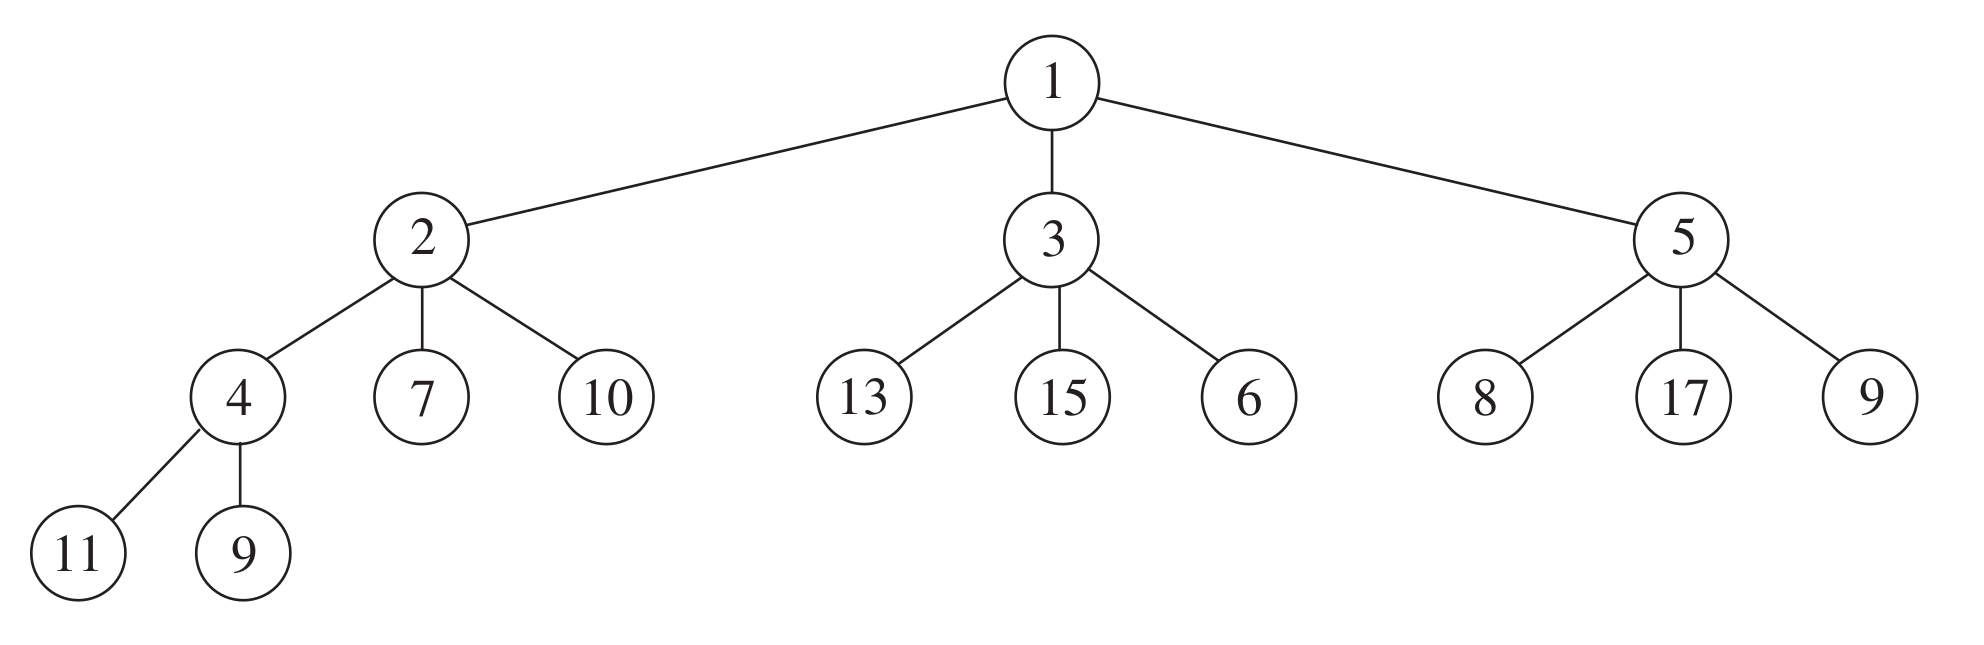
\includegraphics[width=0.9\textwidth]{images/d_3_heap.png}
  \caption{一个 $3-$堆。}
  \label{fig::3-heap}
\end{figure}

在这种情况下，$d-$堆可以像B树一样具有优势。最后，有证据表明 $4-$堆在实践中可能优于二叉堆。

除了无法执行查找操作外，堆实现最明显的弱点是将两个堆合并为一个是一个困难的操作。这意味着将两个优先队列合并成一条优先队列，这是一个合理的需求。
这个额外的操作被称为合并。有相当多的方法可以实现堆，使得合并操作的运行时间为\(O(\log N)\). 
我们现在将讨论三种不同复杂度的数据结构，它们有效地支持合并操作。我们将把任何复杂的分析推迟到第 11 章。

\subsection{左堆（Leftist Heaps）}

设计一个数据结构，既能高效地支持合并（即在\(O(N)\)时间内处理合并），又只能使用数组，这似乎很难，就像在二叉堆中一样。
原因是合并似乎需要将一个数组复制到另一个数组中，这将花费\(\Theta(N)\)时间来处理等大小的堆。
出于这个原因，所有支持高效合并的高级数据结构都需要使用链式数据结构。在实践中，我们可以预期这将使所有其他操作变慢。

像二叉堆一样，左堆既有结构属性也有排序属性。实际上，左堆和几乎所有使用的堆一样，具有我们已经看到的相同的堆序属性。
此外，左堆也是二叉树。左堆和二叉堆之间唯一的区别在于左堆不是完全平衡的，而是实际上尝试非常不平衡。

左堆, 也有翻译成左倾堆(左派, 左倾主义者, leftist). 它的出现是为了解决
高效率合并的问题. 一般而言, 两个带序关系的数据结构合并, 最优也是
$\Theta(n)$ 的代价. 很难想像, 在合并的时候, 能够不将两个输入的结构体读
一遍. 然而, 确实有这样一种结构, 能够突破这个上限. 当然, 为此我们也需要
付出一定的代价, 我们不能再以数组存储我们堆, 而必须用链接构建的二叉树来
实现我们的结构.

\subsubsection{左堆属性}

我们定义任何节点X的空路径长度（null path length，npl(X)）, 为从 X 到没有两个子节点的节点的最短路径的长度。
因此，没有子节点或只有一个子节点的节点的空路径长度为 0, 而 npl(null ptr) $= -1$. 在图 6.20 中的树中，空路径长度在树节点内部标出。

请注意，任何节点的空路径长度都比其子节点的空路径长度的最小值多 $1$. 这适用于子节点少于两个的节点 因为 nullptr 的空路径长度为 $-1$.

左堆属性是，对于堆中的每个节点 X, 左子节点的空路径长度至少与右子节点的一样大（不许右边更大）。这个属性只在图 6.20 中的一棵树上得到满足，
即左边的那棵树。这个属性实际上特意确保树是不平衡的，因为它明显地使树向左深入（左边更大）。实际上，由一系列左节点组成的长路径的树是可能的
（实际上为了便于合并，这是可取的）—— 因此得名左堆。

\begin{figure}
  \centering
  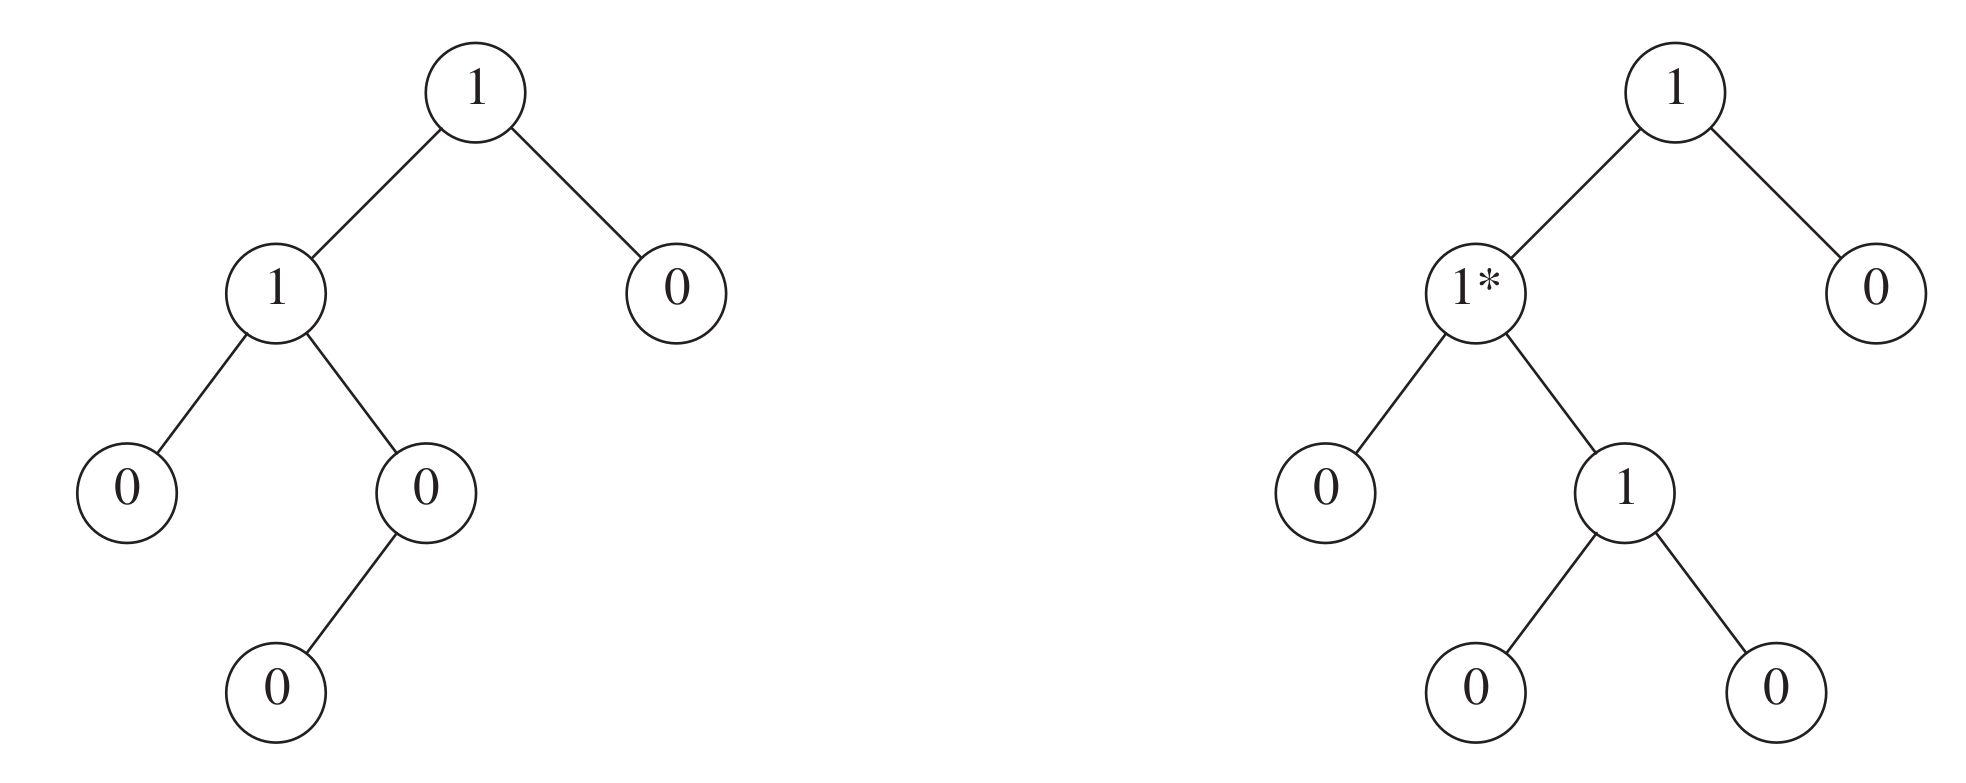
\includegraphics[width=0.9\textwidth]{images/npl.png}
  \caption{两颗树的 npl, 只有左树是左堆。}
  \label{fig::leftist_heap}
\end{figure}

因为左堆往往有深入的左路径，所以右路径应该是短的。实际上，左堆中的右路径与堆中的任何路径一样短。否则，将会有一条通过某个节点 X 并采取左子节点的路径。
那么 X 就会违反左属性。

% 左堆是一个二叉堆, 它在序关系上和二叉堆一致. 但是并不要求是完全二叉树.
% 顾名思义, 它要求整棵树向左倾斜, 而不是平衡. (它是一棵反平衡树.) 为了正
% 确定义左堆, 我们需要首先引入一个定义:

% \noindent{\bf 空路径长度(null path length, npl)} 一个节点 $X$ 的空路径
% 长度, $\mathrm{npl}(X)$, 是从该节点到第一个没有两个孩子的后代节点的路
% 径长度. 特别地, 不到两个孩子的节点的空路径长度是 $0$, 而空节点的空路径
% 长度是$-1$. 一般地, 一个节点会比它的孩子的空路径长度多 $1$.

% \noindent{\bf 左堆(leftist heap)} 左堆是一个二叉堆(不要求满), 且对它的
% 任意节点, 它左孩子的空路径长度不短于右孩子.

因为左倾, 所以左堆的右路径都相对较短. 因此我们通过将一些实质操作放在右
边, 从而实现降低复杂度的目的.

{\bf 定理} 如果一个左堆的右路径上有 $r$ 个节点, 则它总共至少有 $2^r -
1$ 个节点.

用数学归纳法不难证明. 

\subsubsection{左堆的基本操作}

首先我们指出, \verb|insert| 可以看作 \verb|merge| 操作, 如果你把一个节
点也看作一个堆. 而 \verb|deleteMin| 则不难通过删除 \verb|root| 节点,
再将左右子树(都是堆)合并实现(合并成一个堆). 所以让我们集中精力来讨论
\verb|merge| 操作. (所有核心操作都可以通过 \verb|merge| 实现.)

其实 \verb|merge(H1, H2)| 操作也很简单, 我们用递归的语言讲, 就是:

\begin{enumerate}
\item 如果 \verb|H1| 或 \verb|H2| 是空堆, 则返回另一个；
\item 比较 \verb|H1| 和 \verb|H2| 的 \verb|root|, 不妨设 \verb|H1| 的
  根节点更小, 则将 \verb|merge(H2, H1.right)| 作为 \verb|H1| 的右子树.
\item 如果 \verb|H1| 的右子树的 \verb|npl| 更长, 则交换 \verb|H1| 的左右子树.
\item 更新 verb|H1| 根节点的 \verb|npl|.
\end{enumerate}

这是一个自然语言描述, 请对比课本 Fig 6.27 理解. 

在结构上, 我们需要在每个二叉树节点中增加一个属性存放 \verb|npl| 值, 并
及时更新这个属性. 这种通过增加一个额外属性, 并保持这个属性来维持数据结
构的某种特性, 是复杂数据结构设计中常见的一种手段(扩展数据结构,
argumenting data structure), 比如 Avl Tree.

\subsection{斜堆(Skew Heaps)}

就像有了 AVL Tree, 人们还搞了一个简化版的伸展树(splay tree)一样, 面对
左堆这样的复杂结构, 在划水摸鱼的思想指导之下, 人们设计出了斜堆(skew
heap), 一种自适应调整的左堆. 斜堆是一种二叉堆, 在序关系上和堆一致, 但
不同于左堆, 斜堆不需要保持像 npl 这样的特殊结构(和 Splay Tree 一个逻辑),
因此它做不到确保右路径充分短, 因此它的操作的最坏可能性是 $\Theta(n)$
的, 但是类似与伸展树, 它的摊还效率,也就是 $m$ 个连续操作的平均效率, 能
够做到 $\Theta(\log n)$. 与此同时,它的结构和操作, 都比左堆要简单很多.

左堆实现的关键是在 \verb|merge| 操作时, 我们总是判断左右子树的
\verb|npl|, 然后决定是否要交换左右子树. 然而在斜堆, 我们在每一个递归操
作中, 不再去做判断, 而是总是交换左右子树. (套路总得人心.)

\subsection{二项队列(Binomial Queues)}

二项队列比较特殊, 它不再是一个优先队列, 而是一个满足堆序关系的树的集合.
或者又可以称为: {\bf 森林(forest)}. 其中的每一棵树, 都是一种被称为{\bf
  二项树(binomial tree)}的数据结构.

\noindent{\bf 二项树(binomial tree)}: 高度为 $0$ 的二项树 $B_0$ 就是一
个节点. 高度为 $k$ 的二项树 $B_k$, 它的子树分别为: $B_0, B_1, \cdots,
B_{k - 1}$. 因此 $B_k$ 的高度就是 $k$, 而它的节点数是 $2^k$ 个:
$$ 
1 + \sum_{i = 0}^{k - 1} 2^i = 2^k.  
$$
而 $B_k$ 中深度为 $d$ 的节点总数, 是 $k \choose d$ 个. 也就是二项系
数.

\begin{center}
  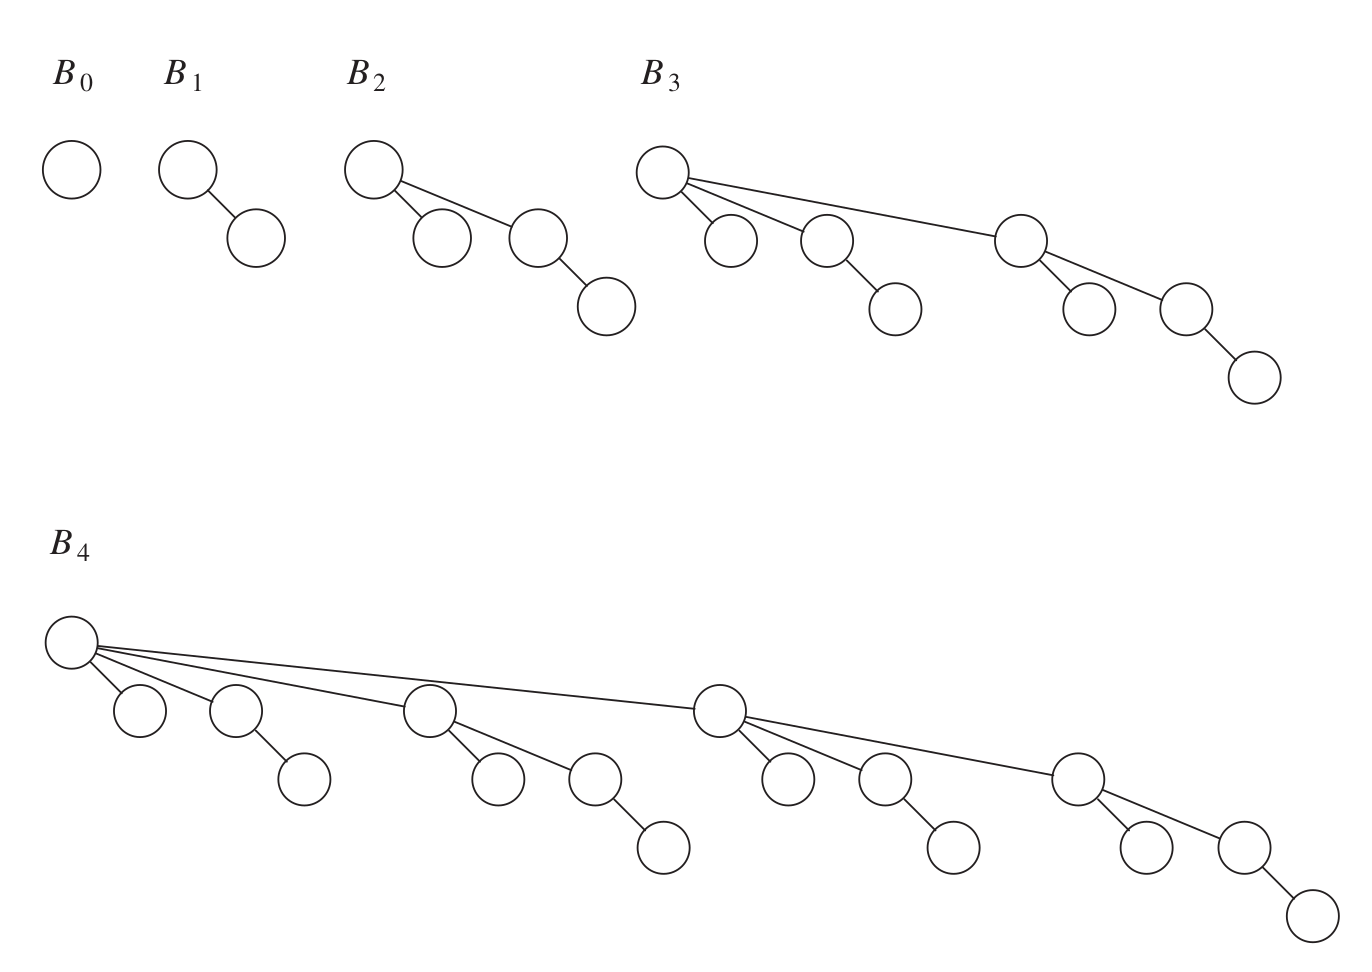
\includegraphics[width=0.9\textwidth]{images/B-heap.png}
\end{center}

如果我们在二项树上应用堆序关系, 并且每一个高度只允许一棵二项树(本质上
就是不考虑各子树的次序, 或者规定一种唯一次序, 比如从左到右为从低到高),
那么我们就有了一种优先队列的实现方法. 要看一个具体长度的优先队列, 由怎
样的二项树构成其实是非常简单且高效的. 比如, 如果一个优先队列的长度是
$13$, 那么首先看它的二进制表示
$$
(13)_{10} = (1101)_2,
$$
于是构成这个有限序列的二项树集合就由 $B_3$, $B_2$ 和 $B_0$ 构成（从低到高）. 分别
对应了二进制表示的非零位. 因此对于 `size` 为 $n$ 的优先队列, 其二项树
集合的具体构成是唯一的. Fig 6.35 给出了一个六个节点（$110$，因此有 $B_1$ 和 $B_2$）组成的二项堆的例子. 

\begin{center}
  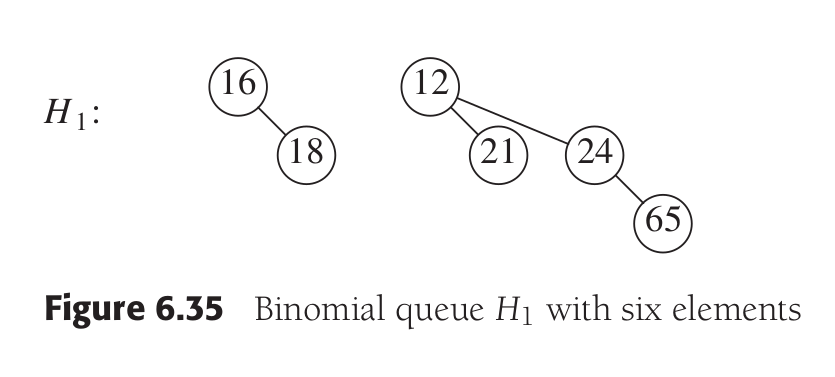
\includegraphics[width=0.9\textwidth]{images/B-tree.png}
\end{center}

\noindent{\bf 二项序列的操作}

最小元素一定出现在全部二项树的根节点, 由于二项树的总数是 $\log n$(二进
制表示). 所以全部搜索一遍的代价也是 $\log n$. 或者, 我们增加一个标记,
记住最小值所在的位置, 并且在动态操作时记得更新, 那么我们就能把这个代价
降到 $\Theta(1)$. 在这种结构下, \verb|merge| 操作变得非常简单. 本质上
就是一个二进制加法的实现. 比如 \verb|H3 = merge(H1, H2)|, 对 \verb|H1|
和 \verb|H2| 的第 \verb|k| 位, 如果 \verb|H1| 和 \verb|H2| 都没有
$B_k$, 那么 \verb|H3| 的第 \verb|k| 位必然没有；如果 \verb|H1| 和
\verb|H2| 中只有一个有 $B_k$, 那么 \verb|H3| 的第 \verb|k| 位就是这个
$B_k$; 如果 \verb|H1| 和 \verb|H2| 的第 \verb|k| 位都有 $B_k$, 那么首先
合并这两课树, 方法是 \verb|root| 小的一个做 \verb|root|, 另一个变成新
树的 $B_k$ 子树, 合并后的子树变成 $B_{k + 1}$, 而将第 $k$ 位空出来. 这
不就是进位么? 进位之后,最复杂的一种情况是原本 \verb|H1| 和 \verb|H2|
的第 \verb|k + 1| 位都有 $B_{k + 1}$. 这种情况, 我们先合并 \verb|H1|
和 \verb|H2| 的 $B_{k + 1}$, 形成 \verb|H3| 的$B_{k + 2}$, 空出的
\verb|k + 1| 位用刚才进位上来的 $B_{k + 1}$ 替换.  Fig 6.35 - 6.38 演
示了一个具体的合并例子.  显然, 两棵二项树的合并是一个$\Theta(1)$ 的代
价, 因此合并两个二项堆是一个 $\Theta(\log n)$ 的动作.

和前面描述的一样, \verb|insert| 本质上就是一个 \verb|merge| 的特例. 因
此单个 \verb|insert| 操作是一个最坏 $\Theta(\log n)$ 的动作. 更加精确
地, 如果一个被插入的二项堆, 它的最小的缺失的子树是 $B_i$, 那么它的插入
步数就是 $i + 1$ (一直进位直到第 $i$ 位, $i$ 从零开始). 由于每一位不存
在的概率都是 $0.5$, 因此总期望是:
$$
E[T] = \sum_{i = 0}^\infty (i + 1) * \left(\frac{1}{2}\right)^{i +
  1} = 2.
$$
令
$$
S = \sum_{k = 1}^\infty \frac{k}{2^k},
$$
则
$$
\frac{S}{2} = \sum_{k = 1}^\infty \frac{k}{2^{k + 1}},
$$
所以
$$
S - \frac{S}{2} = \frac{S}{2} = \sum_{k = 1}^\infty \frac{1}{2^k} = 1,
$$
故
$$
S = 2.
$$
也就是说, 对平均情形, \verb|insert| 是一个 $\Theta(1)$ 的动作. (这是
第一次严格证明平均情形代价.)

进一步, 从空堆开始, 连续的 $n$ 个 \verb|insert| 是一个 $\Theta(n)$ 的
操作. 它只需要 $n - 1$ 次比较. 严格证明是一项作业, 即习题 6.33.

%我们在此题基础上提供一道选做作业, 完成的同学可以额外获得 $0 \sim 10$
%的平时成绩.

Fig 6.39 - Fig. 6.45 给出了一个从空树开始连续 \verb|insert| 的例子.

而 \verb|deleteMin(H)| 操作, 则是先找到最小的 \verb|root|, 然后把其他
的子树全部并成 \verb|H'|(这个代价很低), 将最小 \verb|root| 所在子树,
除去 \verb|root| 之后的全部子数都并作 \verb|H''|(同样代价很低), 然后
\verb|merge(H', H'')| 就可以了. 查找最小 \verb|root|, 建立 \verb|H'|
和 \verb|H''| 以及合并都是 $\Theta(\log n)$ 的动作,因此总代价是
$\Theta(\log n)$.

\begin{center}
  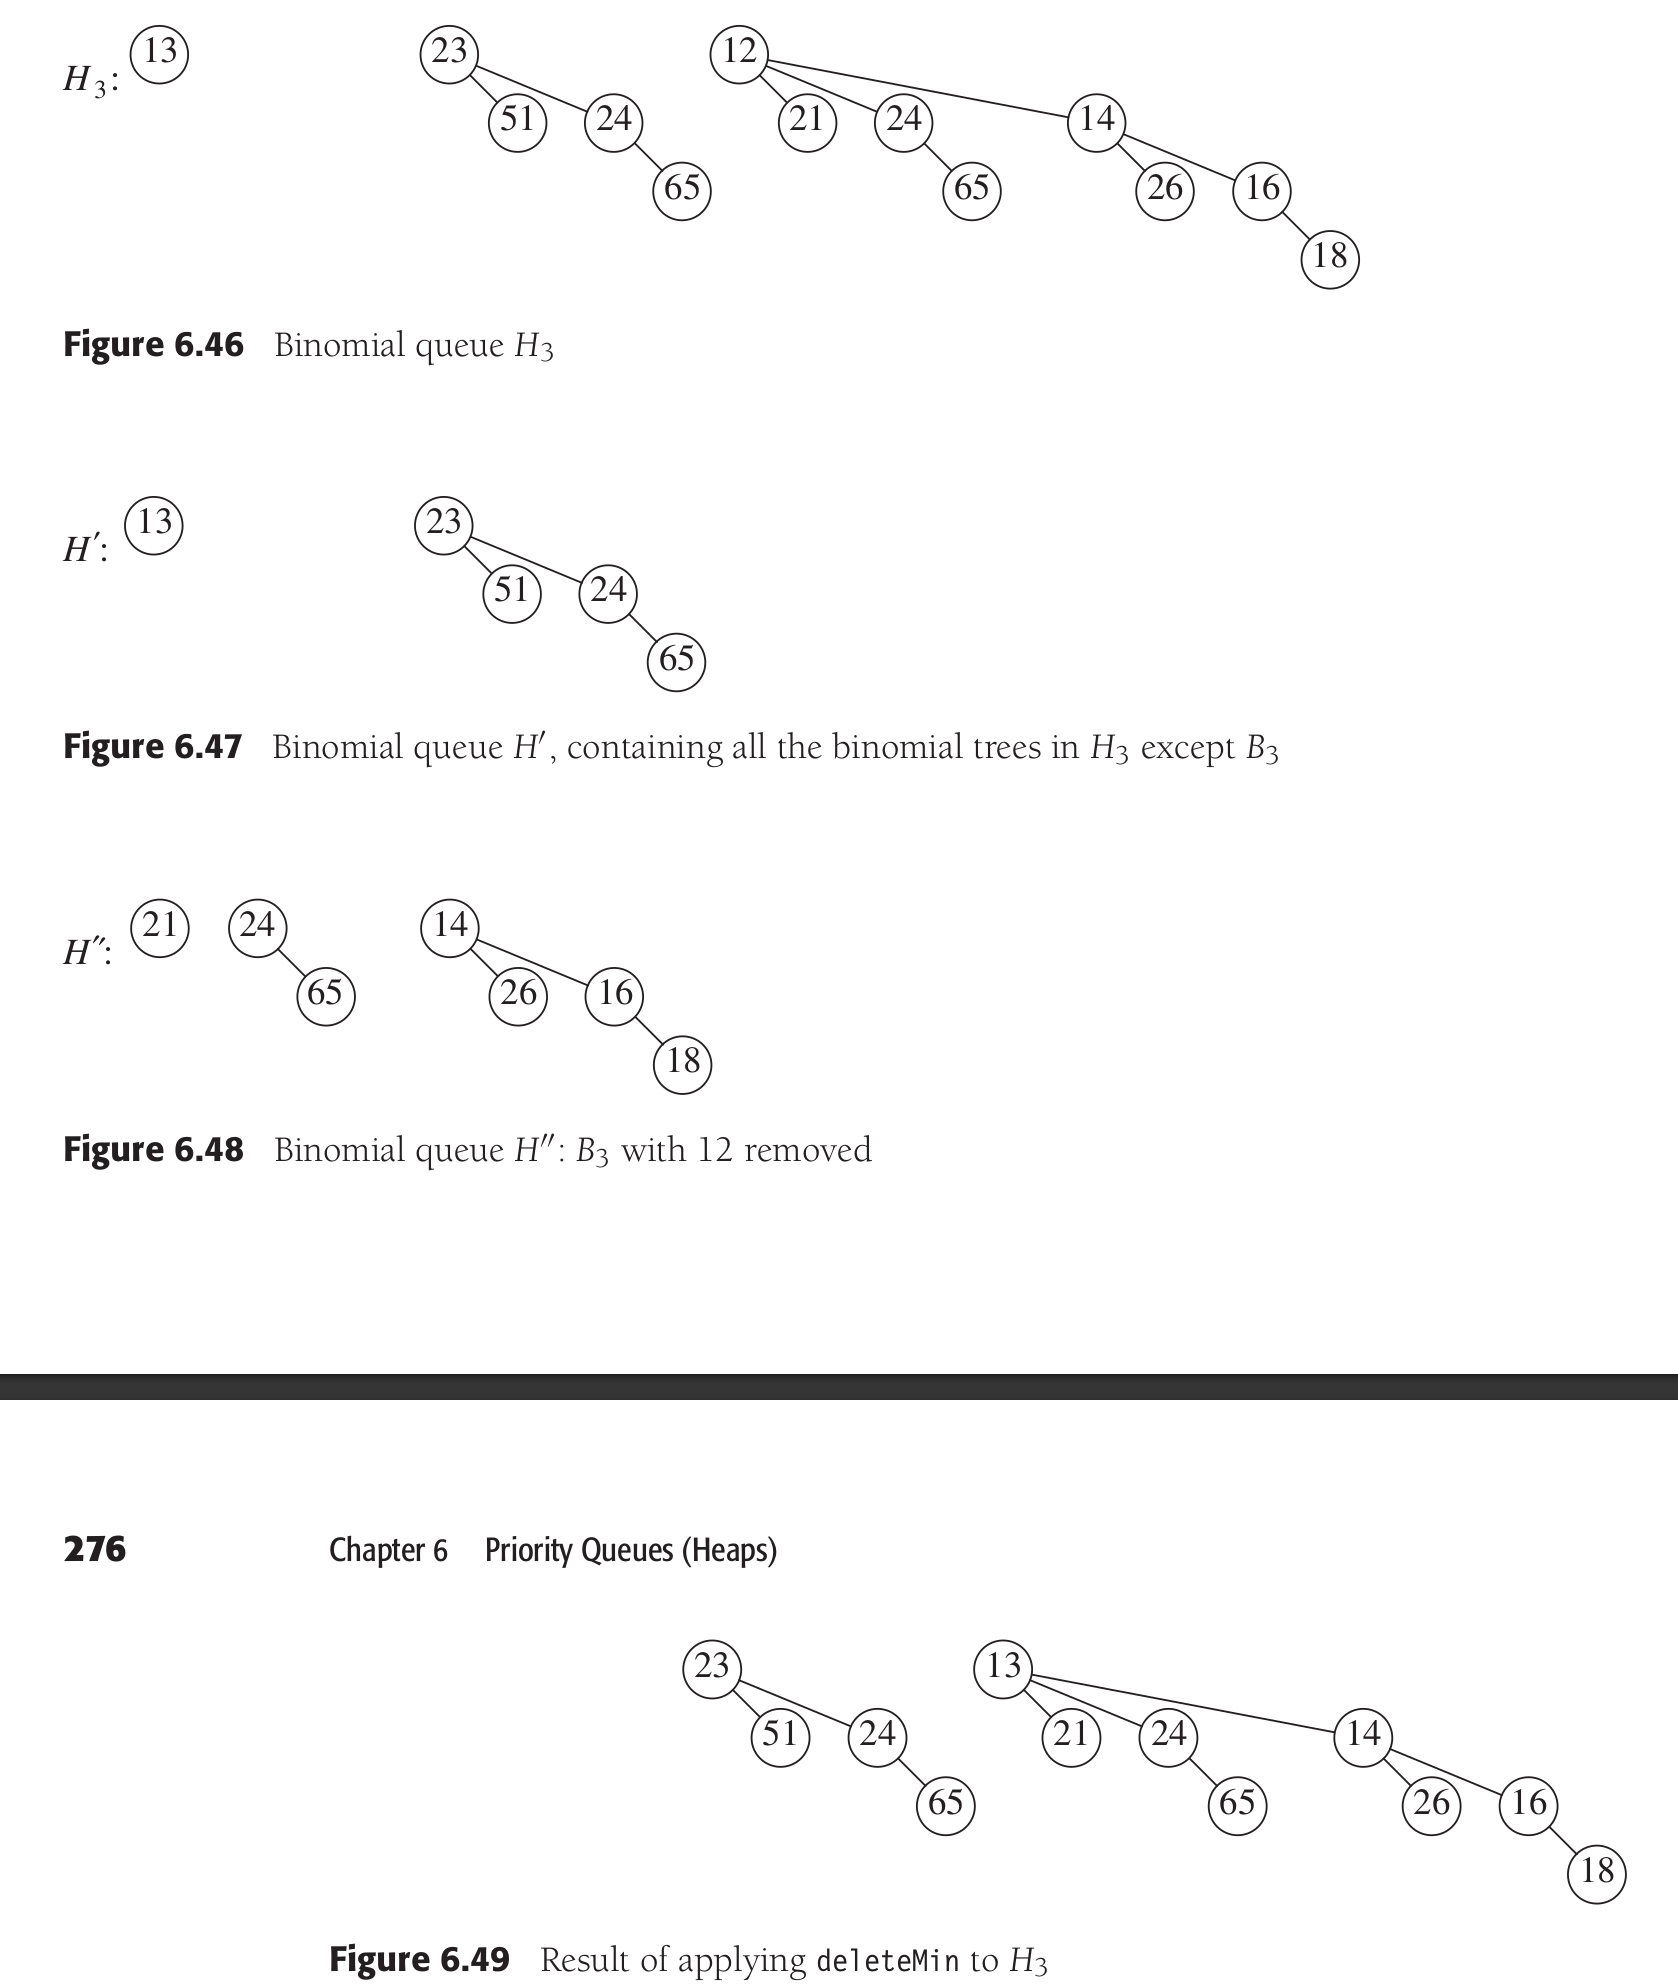
\includegraphics[width=0.9\textwidth]{images/delMin_B_tree.png}
\end{center}
%二项堆的具体实现请阅读 6.8.3 节. 并完成作业. 注意选做作业难度高于此作
%业, 潜在的分值也高, 因此做了选做作业的同学, 可以不做本作业. 这个由大家
%对自己的平时成绩的评估和水平的评估决定.

\section{排序算法}


这一章, 我们来讨论算法中最重要的问题: 排序, 没有之一. 

\noindent {\bf 排序(sorting)} : 输入的一系列元素, $a_0, a_1, \cdots,
a_{n - 1}$, 输出 $a'_0, a'_1, \cdots, a'_{n - 1}$ 为输入数组的一个重排.
且满足 $a'_0 < a'_1 < \cdots < a'_{n - 1}$.

在讨论算法的时候, 我们一般将排序元素视为整数, 以简化我们的细节, 并且一
般不考虑有重复元素出现. 而在具体算法实现时, 利用模板, 我们很容易将算法
扩展至一切有序元素, 并且序关系 $<$ 也可以给予抽象.

我们事实上已经接触了多个排序算法. 这些算法无一例外, 都需要用到序关系,
或者说, 比较运算 $<$. 因此被称为 \textbf{基于比较的排序算法(comparison-based
sorting)}.

下面介绍一些实现简单, 效率不是那么高的排序算法, 但它们可以成为更先进算
法的基础.

\subsection{简单排序算法}

\noindent{\bf 插入排序(insertion sort)} 假设 $a_0, a_1, \cdots, a_{p - 1}$
已经有序, 令 $t = a_{p}$, 从 $i = p - 1$开始, 若 $a_i < t$, 则 $a_{i +
  1} = a_i$(右移), 否则 $a_{i + 1} = t$, 结束.  $i$ 每次减 $1$, 直至 $i = 0$
还未停止, 则 $a_0 = t$. 结束.

我们直接看代码实现: Fig 7.2. (debug) 以及可以利用 STL 框架提供各种接口.
Fig 7.3, Fig 7.4. 这里 \verb|std::move| 的作用有两个: 
\begin{enumerate}
  \item 避免额外复制, 因此数组元素可能很大; 
  \item 避免原始被修改, 因为改成了右值引用. 
\end{enumerate}

显然这是一个 $\Theta(n^2)$ 代价的排序算法. 具体证明太简单不介绍, 自己
看. 

在数字数组中, 逆序对是指任何满足性质 $i < j$ 但 $a[i] > a[j]$ 的有序对 $(i, j)$. 
(行列式) 在上一节的示例中, 输入列表 $34, 8, 64, 51, 32, 21$ 有九个逆序对, 
即 $(34, 8)$, $(34, 32)$, $(34, 21)$, $(64, 51)$, $(64, 32)$, 
$(64, 21)$, $(51, 32)$, $(51, 21)$ 和 $(32, 21)$. 
请注意, 这恰好是插入排序隐式执行的交换次数. 这总是成立, 
因为交换两个彼此相邻但位置不对的元素会消除一个逆序对, 而有序数组没有逆序对. 
由于算法涉及 $O(N)$ 其他工作, 插入排序的运行时间是 $O(I + N)$, 
其中 $I$ 是原始数组中逆序对的数量. 因此, 如果逆序对的数量是 $O(N)$, 
那么插入排序的运行时间是线性的. 

我们可以通过计算排列中平均逆序对的数量来计算插入排序的平均运行时间的精确界限, 
和往常一样, 定义平均值是一个困难的命题. 我们将假设没有重复元素 
(如果允许重复, 甚至不清楚重复的平均数量是多少). 在这种假设下, 
我们可以假设输入是前 $N$ 个整数的某个排列 (因为只有相对顺序很重要), 
而且它们都是等可能的. 在这些假设下, 我们有以下定理:

\hl{定理 7.1} $N$ 个不同元素的数组中平均逆序对的数量是 $N(N - 1)/4$.

\begin{proof}
对于任何具有元素的列表 $L$, 考虑 $L_r$, 即倒序排列的列表, 
示例的倒序列表是 $21$, $32$, $51$, $64$, $8$, $34$. 
考虑列表中任意两个元素 $(x, y)$, 代表一个逆序对, 要么在 $L$ 中, 或者在 $L_r$ 中.  
列表 $L$ 及其倒序的列表 $L_r$ 中这样的有序对的总数是 $N(N - 1)/2$ 
($N \choose 2$). 
因此, 一个平均列表有这个数量的一半, 或者有 $N(N - 1)/4$ 个逆序对.   
\end{proof}

这个定理暗示着插入排序平均情况下是二次的。它还对仅通过交换相邻元素进行排序的任何算法提供了一个非常强的下界。

\hl{定理 7.2} 任何通过交换相邻元素进行排序的算法, 在平均情况下需要 $\Omega(N^2)$ 
的时间. 

\begin{proof}
平均逆序对的数量最初是 $N(N - 1)/4 = \Omega(N^2)$. 每次交换只消除一个逆序对, 
因此需要 $\Omega(N^2)$ 次交换.
\end{proof}  

说起来很令人惊讶, 人类在这个代价上徘徊了很久, 才想到一些更好的排序
算法. 其中之一就是 Donald Shell(1914 - 2015) 提出的希尔排序
(Shellsort). 这个算法突破了 $\Theta(n^2)$, 但仍然没有达到最优. 不过由
于代码简单, 在规模不是很大的场合, 仍然有人采用. 而且很多先进算法, 是在
其基础之上发展出来的.

\noindent {\bf 希尔排序(Shellsort)} 这个算法的关键是等距间隔排序. 比如
先对 $a_0, a_7, a_{14}, \cdots$ 排序, 然后再对$a_0, a_3, \cdots$ 排序,
当最后对间隔 $1$, 也就是 $a_0, a_1, \cdots$ 排序结束之后, 显然就是最后
结果. 这么做能够加速的关键是, 对插入排序而言, 最好的情形是已经有序. 当
先进行 $h_l$ 间隔排序, 后进行 $h_s$ 间隔排序, 且 $h_l > h_s$ 时, 后一
次排序不会打乱第一次排序的次序, 而且前一次排序会导致后一次排序时, 待排
序列部分已经有序. 因此能起到加速的作用.

因此我们需要构建递增序列 $h_1, h_2, \cdots, h_t$, 一般 $h_1 = 1$. 我们
将间隔从 $h_t$ 下降到 $h_1$, 每一次间隔排序采用插入排序, 就得到希尔排
序. 由于最后一次总是 $h_1 = 1$, 所以我们要确保进行最后一次排序前, 数组
尽可能已经有序. 这里不同的递增序列 $\{h_k\}$ 会影响排序效率. 书上介绍
了几种可以选择的序列, 序列的挑选原则是元素 $h_k$ 应该彼此互素. 当年希
尔给出的却是代码 Fig 7.6 的策略, 不断地 2 分降低似乎看上去很自然, 实际
效果却很差, 比如 Fig 7.7 给出了一个极端例子, 当 $h_k = 2^k, k = 0, 1,
\cdots$ 时, 希尔排序比插入排序更慢(此时 $h_1 = 1$ 完全就是插入排序, 之
前则全员摸鱼).

为此 Hibbard 建议使用奇数序列, 这反而能使最坏效率提升至 $\Theta(n^{3 /
  2})$. 证明见课本定理 7.4. 这个实际操作的例子其实就是 Fig 7.5.

课本中说, 目前实际操作中已知的最好序列是:
$$
\{1, 5, 19, 41, 109, \cdots\}
$$
它们是
$$
h_k = \left\{
\begin{array}{ll}
  9 \cdot 4^i - 9 \cdot 2^i + 1, & \mbox{$i$ 是偶数},\\
  4^{i + 1} - 6 \cdot 2^i + 1, & \mbox{$i$ 是奇数}.
\end{array}
\right.
$$
这里 $i \geq 0$. 但是对它的证明, 以及是否存在更好的序列, 则是一个开
放问题, 当中涉及到了数论. 这个序列增长很快, 我们可以实现把这个序列算好
存起来.

由于希尔排序很简单 (一个序列, 加上不断地插入排序), 所以在实际工作中也
可以使用. 效果也还行. 但它不是最优的.

\noindent{\bf 堆排序(heapsort)} 

效率最优的排序算法其实我们已经掌握, 就是先建一个堆, 然后逐个
\verb|deleteMin|, 将删除的元素存到另一个输出数组中. 这样就得到一个代价
为 $\Theta(n \log n)$ 的排序算法. 这个算法不但是目前位置我们学过的排序
中最优的, 也可以证明, 在基于比较的排序算法中, $\Theta(n \log n)$ 是最
优下界(后面会讲).

但是这个算法有一个问题, 它需要第二个数组. 这种排序算法称为{\bf 非原地
  的}. {\bf 原地(in-place)性}是排序算法的一个重要性质. 它表示在排序过
程中, 不需要 $\Theta(n)$ 级别的缓存空间. 空间特性也是算法设计时的一个
重要特性,它意味着内存资源的消耗量.

要将堆排序改造成原地的也不是不可能. 如果我们是用数组来实现二叉堆, 每一
次我们做 \verb|deleteMin|, 我们都会空出数组尾部的一个位置. 而这个位置
正好记录输出. 但是如果采用最小堆, 最后的排序结果会是降序输出
(decreasing, 从大到小). 如果我们还是想保持升序(increasing), 那么我们可
以采用最大堆.  (实际上, 最小最大堆可以通过改变 $<$ 的定义来完成, 甚至
模板化.)

由于已经有基础, 我们也不多讲堆排序, 大家自己阅读 7.5 节.

\noindent{\bf 归并排序(mergesort)}

归并排序是一个非原地的排序算法, 它始终需要一个和最终输出数组同样规模的
缓存数组. 此外, 它是一个典型的递归过程.

假设数组 \verb|A| 和 \verb|B| 都是已经已经排序的, 所谓归并就是将这两个
数组合并成一个长度等于 \verb|size(A) + size(B)| 的数组 \verb|C|, 且要
求数组 \verb|C| 也是有序的.

这个过程不难构建, 我们只需同时遍历 \verb|A| 和 \verb|B|. 比如
\verb|iA| 和 \verb|iB| 分别是遍历 \verb|A| 和 \verb|B| 的下标, 那么如
果 \verb|A[iA] < B[iB]|, 则\newline
\verb|C[i] = A[iA], i++, iA++|, \newline
否则 \newline
\verb|C[i] = B[iB], i++, iB++|. \newline
这里 \verb|i| 从 \verb|0| 开始. 注意\verb|A| 和 \verb|B| 会有一个先遍历完,
剩下的元素就只要复制到 \verb|C| 就可以了. 这个过程, 我们可以称为\newline
\verb|merge(A, B, C)|. \newline
但是为了递归, 我们将接口设计成\newline
\verb|merge(A, tmp, left, right, end)|. \newline
这里 \verb|A| 是待排序数组. \verb|tmp| 是缓存数组. 我们在这个过程中, 将\newline
\verb|A[left]... A[right - 1]| \newline
和
\newline \verb|A[right] ... A[end]| \newline
合并到 \verb|tmp| 的对应位置中.

而整个归并排序就可以写成

\begin{lstlisting}[language=C++]
mergesort(A, tmp, left, right)
{
	if (left < right)
	{
		center = (left + right) / 2;
		mergesort(a, tmp, left, center);
		mergesort(a, tmp, center + 1, right);
		merge(a, tmp, left, center + 1, right);
	}
};
\end{lstlisting}

这个过程的关键是归并过程, 我们来手画一个例子. 比如课本 p305 的例子:
24, 13, 26, 1, 2, 27, 38, 15.

对归并排序的效率分析, 是时候祭出我们之前讲过的主定理了. 显然, 整个归并
排序中,
$$
T[n] = 2 T[n / 2] + f(n),
$$
这里 $f(n)$ 就是归并过程, 是一个 $\Theta(n)$ 的代价. 而由主定理, 这里
$a = 2$, $b = 2$, 因此有
$$
f(n) = \Theta(n^{\log_ba}) = \Theta(n),
$$
所以
$$
T(n) = \Theta(n^{\log_ba}\log n) = \Theta(n \log n).
$$

这个结论是严格的(基于主定理的证明). 书上给出了一个递推分析的过程. 结论
相同, 但注意这种递推分析只是一种技巧, 因为当中有归纳总结(猜测)过程, 所
以严格来说, 这个结论要成立, 还必须用数学归纳法严格证明.

我们之前还讲过另一种递归分析技巧, 画递归树. 注意这也是一种归纳技巧, 其
结论不能代替归纳法证明.

\subsection{快速排序(Quicksort)}

这是最重要, 应用最广的一个排序算法. 由 Tony Hoare (C. A. R. Hoare) 于
1962 年 (希尔排序是 1959) 提出. 也一度被认为(我不知道为啥书上这么说)是
最快的排序算法. C++ STL 库中的 sort 算法, 默认就用这种算法.

快速排序, 同样采用了递归设计, 或者说, 在算法设计上, 采用了{\bf 分治策略}
(devide-and-conquer, 老英国正米字旗了...). 其基本想法是, 把一个
规模为 $n$ 的问题, 切割成 $a$ 个独立的规模为 $\frac{n}{b}$ 的子问题. 逐
个解决,再通过合并这 $a$ 个子问题的答案, 得到最终答案. *关键是:* 这个过
程会递归重复, 直到非常简单的基础情形, 能直接得到答案(或者说, 能够在
$\Theta(1)$ 时间得到答案.)

整个分治策略, 一般由 3 个典型阶段构成:

\begin{enumerate}
\item 分解: 比如在归并排序, 每一次分解将输入数组, 对等地分成两个子数组；
\item 治理: 对每个子问题各自解决. 注意这里解决的方法是继续分治.
  所以这个过程会不断重复, 直到出现能在 $\Theta(1)$ 情况解决的最简单情形.
  比如只有一个元素的数组. 
\item 合并: 对两个已经完成排序的子数组, 用 \verb|merge|
  将它们合并成一个有序的数组.
\end{enumerate}
   
以上在程序实现上, 我们可以使用递归实现；而在算法分析上, 我们可以采用主
定理, 或者归纳猜测加归纳证明.

而在快速排序, 这三个过程可以如下描述:

\begin{enumerate}
\item 分解: 对每个输入数组, 寻找它的一个元素作为主元(pivot),
  然后将数组重新排列成: 凡是在主元之前的元素, 都小于等于主元,
  凡是在主元之后的元素, 都大于等于主元(注意, 我们首次强调元素可能重复出现).
  这样我们实际上将输入数组分成了两部分: 小于等于主元的, 和大于等于主元的.
  因此这个过程又被称为分划(partition).
\item 对分划得到的两部分, 各自独立解决. 或者各自重复这个分划过程,
  直到数组非常简单, 比如只有若干个个元素, 可以直接给出顺序. 这是一个递归过程.
\item 快速排序不存在合并过程.
\end{enumerate}

可见, 快速排序的关键在于分划如何实现. 首先的问题是如何选择主元.
书上特别强调, 不要选择第一个元素作为主元. 但为了算法讨论方便,
我们默认第一个元素作为主元. 这样如果你有更好的元素做主元,
在算法实现时, 只要先做一次交换即可.


\begin{lstlisting}[language=C++]
paririon(A, p, q)       /// 将数组 A[p...q] 分解, 注意 A[p] 和 A[q] 都算在内.
    x = A[p];           /// 选择第一个元素做主元
	i = p + 1;          /// 左边的读取位置 
	j = q;              /// 右边的读取位置
	while (i != j)
		while (A[j] >= x && i < j)
			j--;        /// 使 A[j] 右边都大于 x
		while (A[i] <= x && i < j)
			i++;        /// 使 A[i] 左边都小于 x
		if (i < j)      /// 在这个点, 必有 A[i] > x, A[j] < x,
	                    /// 因此如果 i 还在 j 左边, 交换这两个元素
            swap(A[i], A[j]);
	swap(A[p], A[j]);   /// 主元交换到位
	return j;
\end{lstlisting}

这个过程结束的时候, 如果返回值为 \verb|r|, 则有\newline 
\verb|A[p...r - 1] <= A[r] <= A[r + 1...q]|\newline
有了 \verb|partition| 过程, 我们的快速排序就简单了:

\begin{lstlisting}[language=C++]
quicksort(A, p, q)
	if (p >= g)
		return;
	r = partition(A, p, q);
	quicksort(A, p, r - 1);
	quicksort(A, r + 1, q);
\end{lstlisting}

\subsection{快速排序的复杂度}

\noindent{\bf 最好情形: } 每次都能恰好 2 等分, 中间遍历, 分割,
交换是一个 $\Theta(n)$ 过程: 
$$ 
T[n] = 2T[\frac{n}{2}] + \Theta(n), 
$$
由主定理(2), 
$$ 
T[n] = \Theta(n^{\log_ba}\log n) = \Theta(n\log n).  
$$

\noindent{\bf 最坏情形: } 已经排序, 或者逆序. 如果总是选第一个做主元,
则每次都只能将一个子问题规模从 $n$ 降到 $n - 1$, 另一个则什么也不用做,
也即
$$
T[n] = T[0] + T[n - 1] + \Theta(n)
$$
不妨设 $T[0] = 1$, $\Theta(n) = n$, 则
$$
\begin{array}{rcl}
T[n] &=& 1 + T[n - 1] + n \\
&=& 1 + 1 + T[n - 2] + n - 1 + n \\
&\cdots&\\
&=& \sum_{i = 1}^{n} 1 + T[0] + \sum_{i = 1}^n i \\
&=& \frac{(n + 1)(n + 2)}{2} = \Theta(n^2).
\end{array}
$$

所以这就是书上反对总是拿第一个元素做主元的原因. 因为在实际工作中,
一个待排序的数组, 其实是基本有序的这种情况是很常见的.

那么一个偷懒的策略, 是随机挑选一个元素做主元. 这个实现很简单,
我们只要随机抽取一个元素, 将它交换到第一个元素, 然后其他都不变.

那么这么做能否做到, 平均意义上是高效率的呢?

我们先看一个特例:

$$
T[n] = T[\frac{n}{10}] + T[\frac{9}{10}n] + \Theta(n).
$$

也就是说, 假设我们每次抽取, 都恰好使得切割出现在 $\frac{n}{10}$ 的位置.
这是一种极不平衡的情形. 那么在这么不平衡的情形下, 我们能否保持高效率? 

我们采用更直观的递归树来分析.

从递归树我们可以看出, 只要不出现极限情形, 对于一般常数意义下的严重不平
衡, 快速排序仍然是高效的. 更严格的期望证明, 参见 MIT03.

因此书上首先建议, 一个更好的随机抽取主元方法, 是随机抽取 3 个元素, 然
后取它的中位元素. 

这个方法隐含暗示我们, 如果我们的数组长度小于 3, 就不必继续递归了. 显然,
从刚才的递归树分析, 一个额外得到的直观是, 越接近叶子层, 树越茂密. 所以,
递归在 \verb|n = 3| 退出还是 \verb|n = 1| 退出, 速度上可能会差 $4$ 倍.
因此是可以考虑的. 事实上, 当数组长度小于等于 $3$ 时, 我们只要做若干个\newline
\verb|if... else| 判断即可决定正确的次序. 这是 $\Theta(1)$ 的代价.
书上在 7.7.3 甚至建议对 $n \leq 20$ 做特殊处理.

在考虑了上述细节之后, 我们能够期待一个在操作中实际效率是
$\Theta(n\log n)$ 的快速排序算法. 相比归并排序法, 它是原地的.
而且它实现非常简单. 然而, 这里涉及另一个排序算法的概念: 稳定性. 

\noindent{\bf 稳定性} 如果待排序算法中存在相同的元素,
如果排序之后没有改变相同元素的相对位置, 则称该排序算法是稳定的(stable).
否则, 称不稳定的(unstable).

显然, 归并排序是稳定的, 但是标准的快速排序算法, 是不稳定的.
所以 STL 中的两个排序算法, \verb|sort| 和 \verb|stable_sort|
分别用快速排序和归并排序实现. 如果给快速排序提供缓存空间,
比如记录每个元素在排序后的原始下标. 那么也可以实现稳定,
但是同时也丢失了原地性. 既要又要? 堆排序考虑一下, 但算法更复杂. 

排序的稳定性在多重排序时很有意义. 比如, 先对全部专业课成绩排序,
然后再对英语成绩排序. 我们希望第二次排序不要打乱第一次排序的结果. 

\subsection{比较排序法的最优下界}
我们上面两个算法, 效率的极限都是 $\Theta(n \log n)$. 那么问题是,
还能不能突破这个极限? 回答是, 如果你用了比较运算, 那么这就是最优下界了.
见书上定理 7.7.

这里直观上的理解, 需要用到决策树模型(decision-tree).
也就是对于一个长度为 $n$ 的输入数组, 要完成排序, 需要做几次比较运算?
每一次比较, 都将可能的结果集合做了一个分划, 我们将全部可能的比较,
都用二叉树的形式画出来, 这就是决策树. 任何一个具体的输出, 都是这个决策树的一个叶子.
这是一棵非常茂盛的树, 所以它只是一个思考模型, 不能拿来写程序.
所以我们的问题就是, 这棵树的高度至少也是 $\Theta(n \log n)$.

这个结论其实很显然. 这个树有多少叶子结点? 回答是 $n!$, 全排列.
而一颗高度为 $h$ 的树, 至多也只能容纳 $2^h$ 个节点(完全树).
于是
$$
\begin{array}{r}
n! \leq 2^h \rightarrow h \geq \log n! \geq
\log\left(\frac{n}{e}\right)^n \\ \rightarrow h \geq n \log \frac{n}{e}
= \Omega(n\log n).
\end{array}
$$

注意这里的证明用到了斯特林公式(Stirling's formula):
$$
\lim_{n \to \infty} \frac{n!}{\sqrt{2 \pi n}
  \left(\frac{n}{}\right)^n} = 1.
$$
也就是本质上 $n!$ 是一个指数量:
$$
n! \approx \sqrt{2 \pi n}\left(\frac{n}{e}\right)^n.
$$


\subsection{线性时间排序}

我们已经知道, 比较排序算法的最优下界是 $\Theta(n \log n)$.
所以要突破这个下界, 必须放弃比较. 咋一听这很荒谬, 序关系依赖比较,
所以排序算法似乎无法摆脱比较. 但是, 仔细一想, 序关系对于某些集合, 比如自然数集,
是内禀的属性. 利用这一点, 我们有可能在特定的条件下, 实现线性时间代价的排序.
本质上, 用数数代替比较. 

书上提供了一个称为{\bf 桶排序(bucket sort)} 的算法思路,
其实这是一个计数排序(counting sort). 这两种算法区别不大, 都是线性时间的.
我们先看一下计数排序的伪代码: 设输入
\begin{verbatim}
A[1], A[1], ..., A[N],
\end{verbatim}
都是不超过 \verb|M| 的正整数. 我们构建整数数组 \verb|C[1...M]|,
顺序读取 \verb|A[i]|, 然后用 \verb|C[A[i]]| 来记录 \verb|A[i]| 的个数,
就可以在某种意义上完成了对数组 \verb|A| 的排序.

按这个思路, 我们给出伪代码:

\begin{verbatim}
countingsort(A[1...N], B[1...N], C[1...M])
    for i = 1 to M
        C[i] = 0
    for i = 1 to n
        C[A[i]] = C[A[i]] + 1    /// 依次计算每个 A[i] 的出现次数.
    for i = 2 to k
        C[i] = C[i] + C[i - 1]   /// 计算 1...k 中每一个数最后一次在输出数组中出现的位置.
    for i = n downto 1
        B[C[A[i]]] = A[i]        /// B 存放输出数组.
	C[A[i]] = C[A[i]] - 1    /// C 的递减次序保证了稳定性.
\end{verbatim}
而桶排序可以看作是准备 \verb|M| 个容器, 比如数组 \verb|bucket[1...k]|,
其每一个元素都是数组或链表, 然后将 \verb|A[i]| 逐个 \verb|push_back|
到 \verb|bucket[A[i]]| 中去, 最后统一输出 \verb|bucket| 中全部元素. 

这两个算法都是非原地且稳定的. 看一下计数排序的例子. 

两种算法的计算复杂度都是 $\Theta(N + M)$. 当 \verb|N| 远大于 \verb|M| 时,
可以认为是 $\Theta(N)$ 的.

这两种方法的局限性也很明显, 如果我们要排序的范围很大, 比如,
全部同学的姓名拼音. 那么这个 \verb|M| 就会太大, 以至于不现实.
这里一个很自然的想法是, 我们能不能每次只排一位? 比如如果全部都是 $3$ 位整数,
那么 \verb|M| 也会是 $999$. 但如果我们每次只排一位,
那么就只需要 $10$ 个桶或者计数器. 

一个自然的想法是, 从百, 十, 个, ... 这样从高到低位排序. 然而这是不行的.
幼儿园老师教我们这么做本质上是为了比较大小, 而比较大小我们已经放弃了.
事实上, 百位排序之后, 十位的排序会打乱百位的结果, 使得高位排序毫无意义.
正确的做法是从低到高排序. 也就是, 假设这个数至多 3 位, 那么先按个位排序,
再十位, 再百位. 这里的关键是, 高位排序的结果, 对低位结果的优先级更高.
所以如果我们能在每一位排序中都保持稳定(这里稳定性至关重要),
那么结束最高位排序之后我们就会得到完整的排序结果.

\noindent{\bf 例子.}

这就是 {\bf 基数排序(radix sort)} 的基本思想.

这个想法最早由 Herman Hollerith 于 1890 年提出.
当时的主要目的是为了做人口统计.
1880 年美国的人口已经多到以当时的技术统计一次需要 10 年以上, 但美国宪法规定,
每十年必须完成一次人口统计. 这就尴尬了. Herman Hollerith 设计了一种用于统计的打孔机,
在排序算法上实现了基数排序. 由于效率提升, 即便依靠人工读取, 也使得人口统计可以在短期完成.
从而拯救了美国或美国宪法. Hollerith 的公司经过几次重组之后, 现在仍然存在,
叫 IBM. 这个公司曾经是 PC 的代名词, 事实上, PC 原本就叫 IBM-PC.
直到某一年它把整个计算机硬件部门卖给了联想. 

\subsection{结语}
对排序算法的研究仍然在进行, 比如当数据量非常巨大, 以至于无法在一个存储设备放下时,
该如何高效率排序就是一个在当前环境下值得考虑的问题. 本章最后讨论了这个问题.
一个基本想法是, 归并排序此时仍然有效.


\bibliography{../bibtexlib/crazyfish.bib}
\bibliographystyle{plain}

\end{document}
